\section{Results}
\label{sec:Results}

It can be seen by Figure \ref{fig:ClassDist} that two of the data sets, the  liver and glass, are imbalanced while the third, vowel, has each class equally represented.
Furthermore it is observed that the glass data set is the most imbalanced; this is where the largest increase of performance due to the AdaBoostM1 is expected.
The results of an SVM on the data sets is presented in Section \ref{sec:Results_ParamSearch}.
In Section \ref{sec:Results_AdaBoost} the results are shown for using an ensemble methods.

\subsection{Parameter Search}
\label{sec:Results_ParamSearch}

The parameter search for the optimal C and $\sigma$ parameters is shown in the contour plots of Figures \ref{fig:ParamLiver}, \ref{fig:ParamGlass} and \ref{fig:ParamGlass}.
The liver and glass data set contour plots have many topological features, indicating that small variations in the RBFSVM parameters cause dramatic changes in the accuracy of the trained RBFSVM.
The vowel data set does not display these features but rather has a plateau region atop a precipice in which the accuracy of the classifier does not change dramatically.
The optimal classifier parameters are shown for the coarse parameter search in Table \ref{tab:CoarseParamValues} and for the fine parameter search in Table \ref{tab:FineParamValues}. $C_{min}$ and $C_{max}$ are the starting values of the grid search normalization parameter, $\sigma_{min}$ and $\sigma_{max}$ are the range of kernel size while $C$, $\sigma$ and $\epsilon$ are the optimized normalization parameter, kernel size, and final accuracy respectively.
The values for the fine parameter search were chosen to be 50\% of the optimal values selected by the coarse parameter search.
\begin{table}[h!]
\caption{Coarse Optimal Classifier Parameters}
\label{tab:CoarseParamValues}
\centering
\begin{tabular}{c c c c c c c c}
\hline
\input{../CoarseGridSearchOutput.dat}
\hline
\end{tabular}
\end{table}
\begin{table}[!ht]
\caption{Fine Optimal Classifier Parameters}
\label{tab:FineParamValues}
\centering
\begin{tabular}{c c c c c c c c}
\hline
\input{../FineGridSearchOutput.dat}
\hline
\end{tabular}
\end{table}
\begin{figure*}[!ht]
	\centering
	\begin{subfigure}[b]{0.43\textwidth}
		\centering
		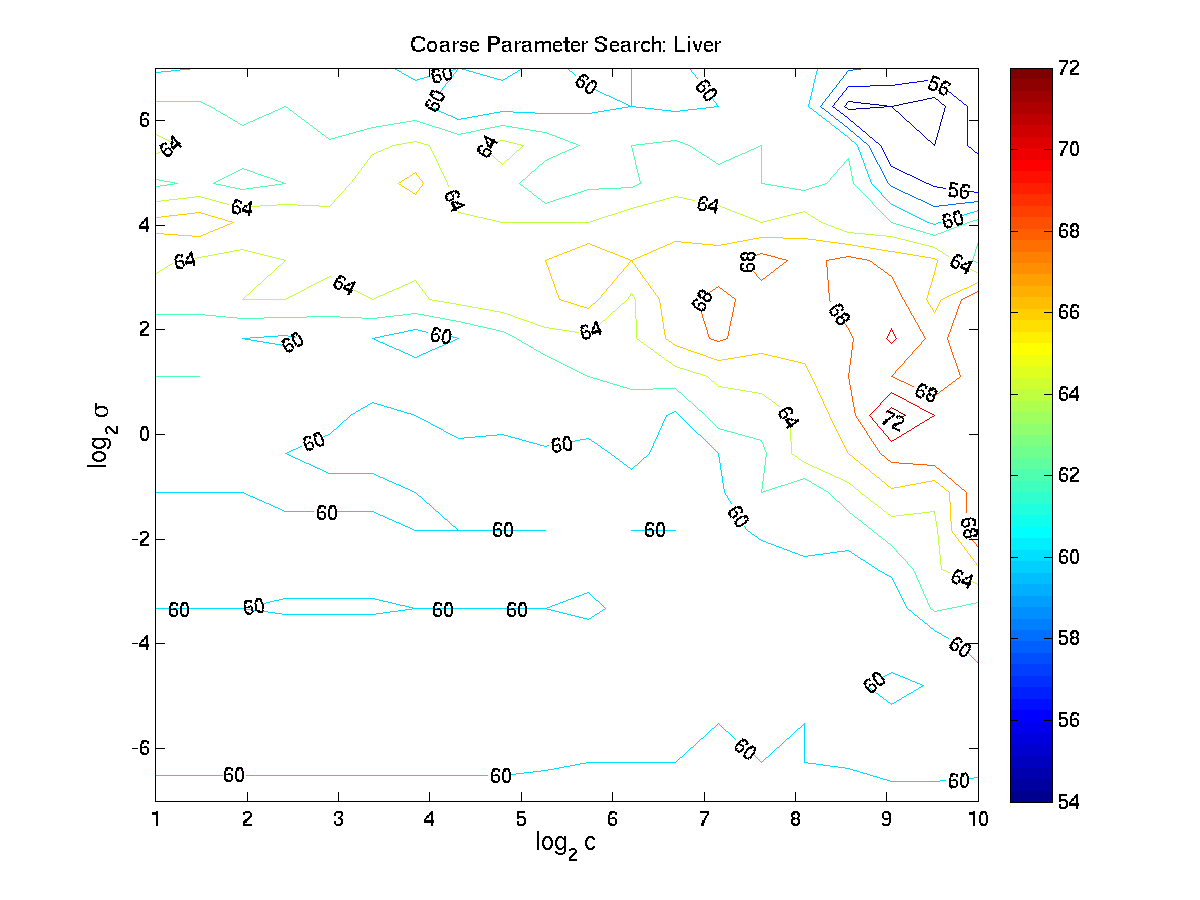
\includegraphics[width=\textwidth]{Liver_coarseSearch}
        \caption{Coarse Search}
	\end{subfigure}%
	~
	\begin{subfigure}[b]{0.43\textwidth}
		\centering
		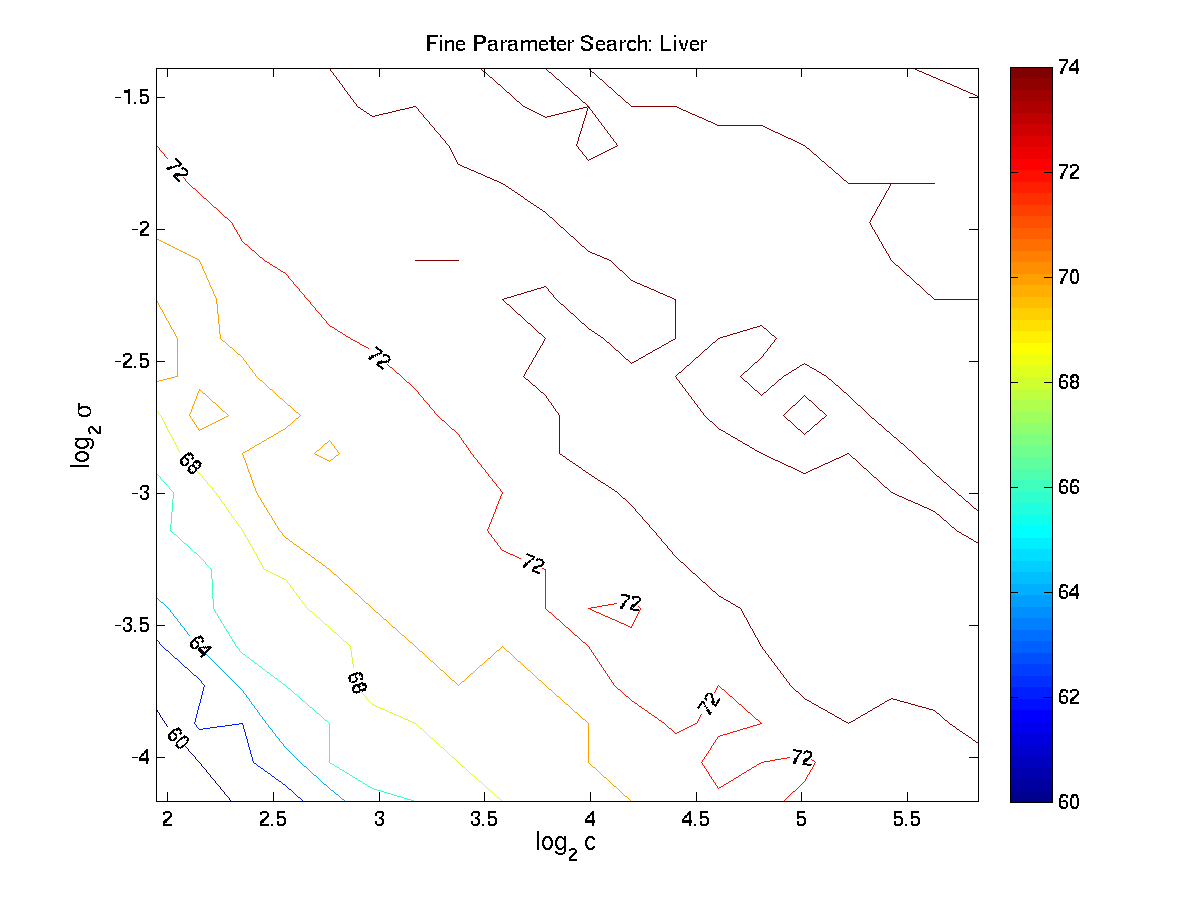
\includegraphics[width=\textwidth]{Liver_fineSearch}
        \caption{Fine Search}
	\end{subfigure}	
	\caption{Parameter search for Liver Disorder}
	\label{fig:ParamLiver}

	\begin{subfigure}[b]{0.43\textwidth}
		\centering
		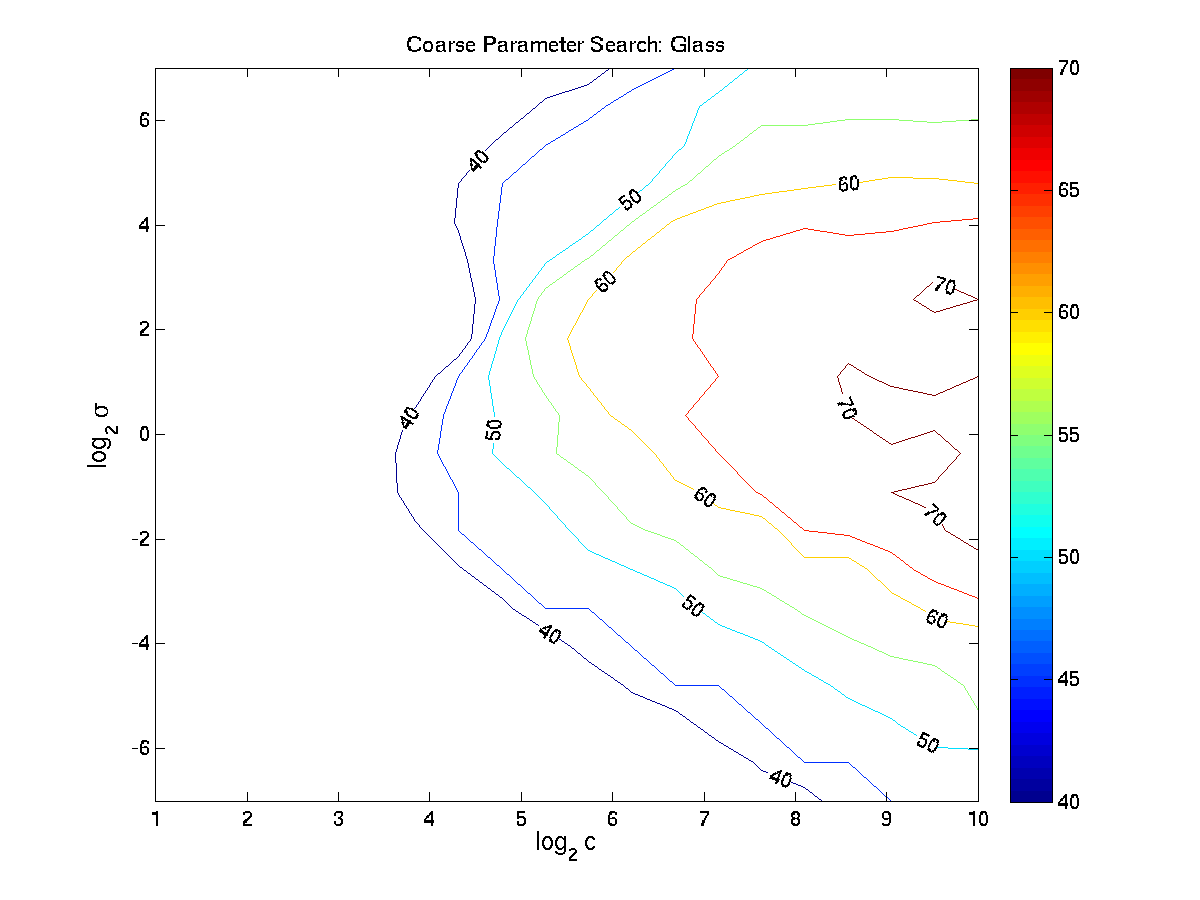
\includegraphics[width=\textwidth]{Glass_coarseSearch}
        \caption{Coarse Search}
	\end{subfigure}%
	~
	\begin{subfigure}[b]{0.43\textwidth}
		\centering
		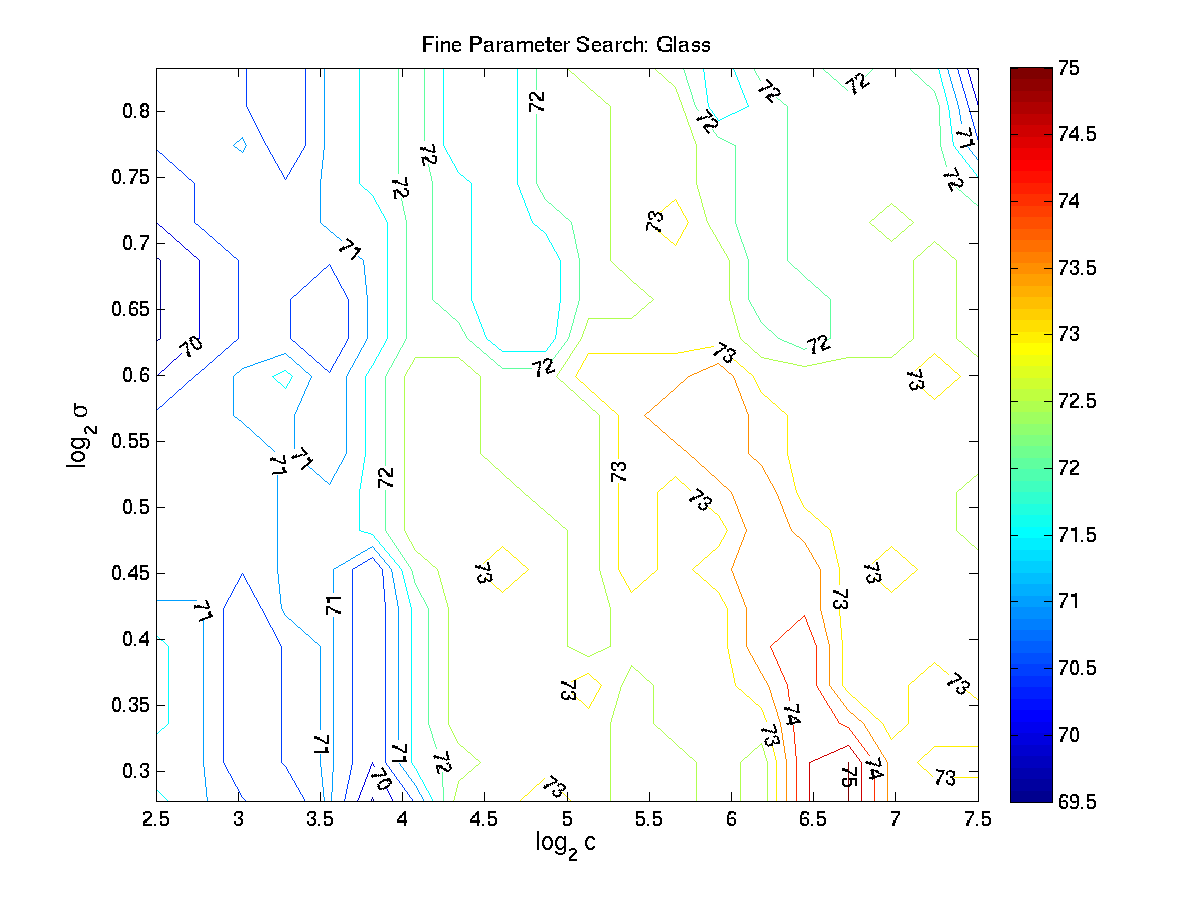
\includegraphics[width=\textwidth]{Glass_fineSearch}
        \caption{Fine Search}
	\end{subfigure}	
	\caption{Parameter search for Glass Disorder}
	\label{fig:ParamGlass}

	\begin{subfigure}[b]{0.43\textwidth}
		\centering
		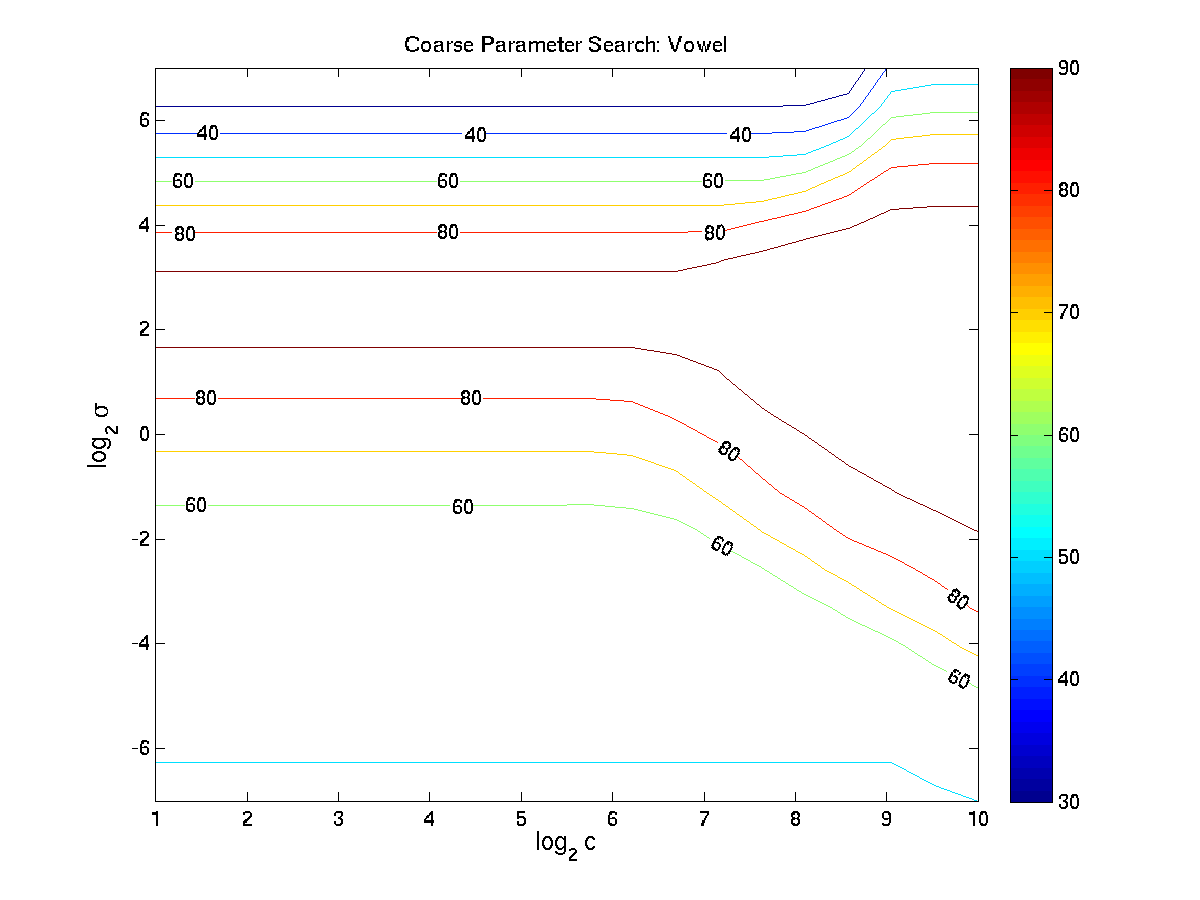
\includegraphics[width=\textwidth]{Vowel_coarseSearch}
        \caption{Coarse Search}
	\end{subfigure}%
	~
	\begin{subfigure}[b]{0.43\textwidth}
		\centering
		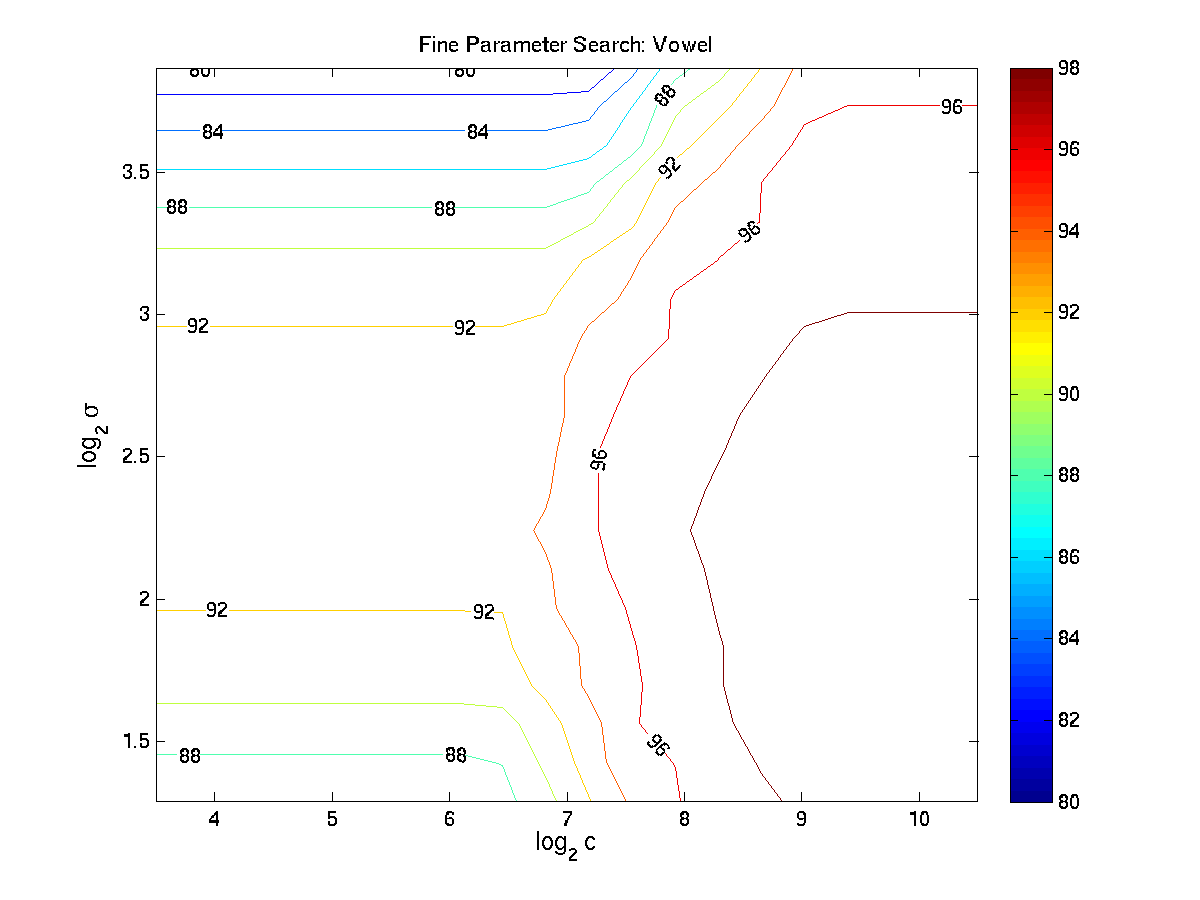
\includegraphics[width=\textwidth]{Vowel_fineSearch}
        \caption{Fine Search}
	\end{subfigure}	
	\caption{Parameter search for Vowel Disorder}
	\label{fig:ParamVowel}
\end{figure*}

The confusion matrices of the RBFSVM classifiers are presented in Tables \ref{tab:SVMConfusionLiver} - \ref{tab:SVMConfusionVowel}.  
\begin{table}[h!]
\caption{Confusion Matrix for RBFSVM (Liver)}
\label{tab:SVMConfusionLiver}
\centering
\input{../Part1_Confusion_Liver.dat}
\end{table}
\begin{table}[h!]
\caption{Confusion Matrix for RBFSVM (Glass)}
\label{tab:SVMConfusionGlass}
\centering
\input{../Part1_Confusion_Glass.dat}
\end{table}
\begin{table}[h!]
\caption{Confusion Matrix for RBFSVM (Vowel)}
\label{tab:SVMConfusionVowel}
\centering
\input{../Part1_Confusion_Vowel.dat}
\end{table}

\subsection{AdaBoostM1}
\label{sec:Results_AdaBoost}
The effect of the number of the classifiers in the ensemble is shown in Figure \ref{fig:AccuracyEnsambleSize}.
It was observed for the un-balanced data sets the number of classifiers is the ensemble did not have a large effect (past a minimum amount of 20).
Furthermore, it was surprising to note that the accuracy of the ensembles was constant for the liver data set, while the vowel data set showed an almost periodic trend that died out as the number of classifiers increased.
The glass data set exhibited significant variation; it is thought that this occurs because of the well in the parameter space (Figure \ref{fig:ParamGlass}).
\begin{figure}[!ht]
    \centering
    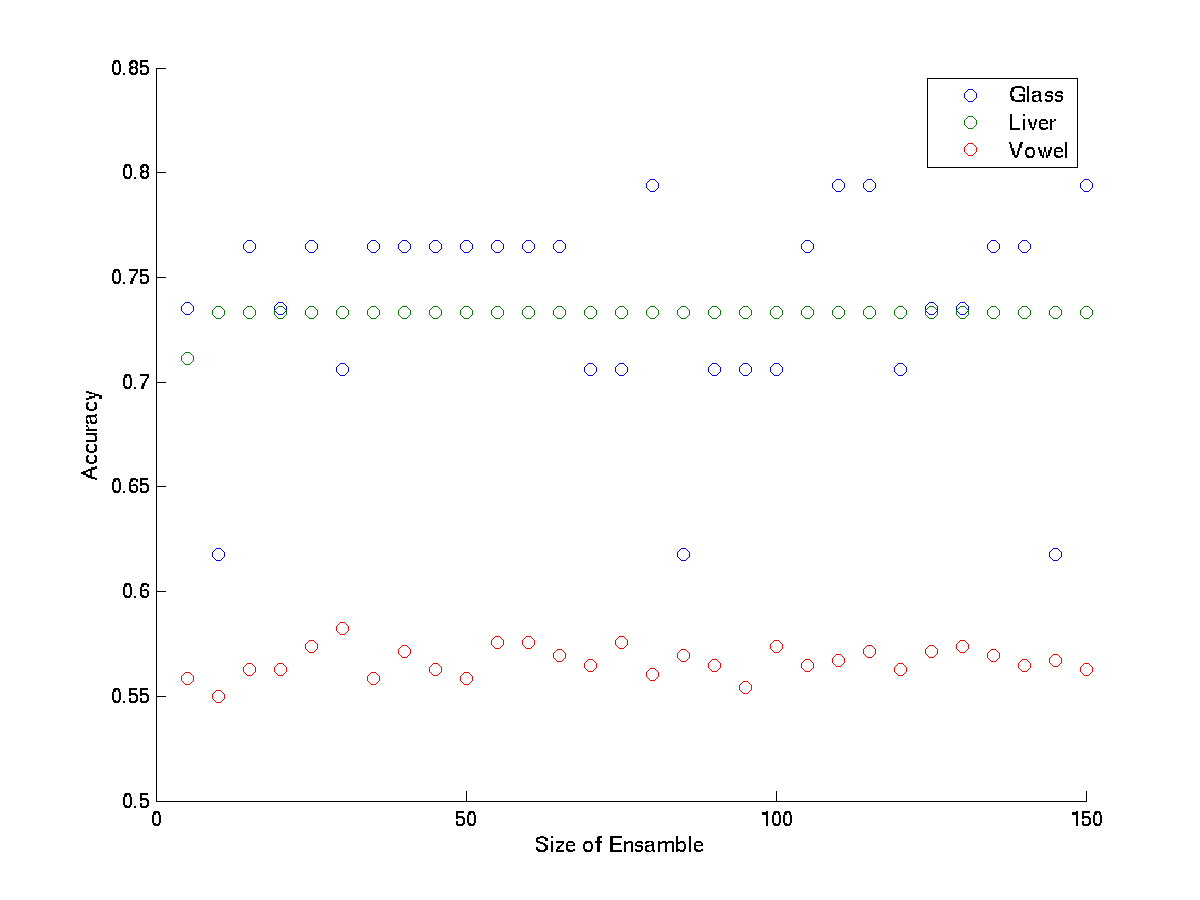
\includegraphics[width=0.45\textwidth]{AccuracyVSEnsambleSize}
    \caption{Accuracy and Number of Components in Ensemble}
    \label{fig:AccuracyEnsambleSize}
\end{figure}

The results using the implemented AdaBoostM1 algorithm are shown below in Table \ref{tab:AdaBoostValues}, while the weights of the individual classifiers (representative of their accuracy) are shown in Figure \ref{fig:EnsambleWeights}.
It is immediately observable that the AdaBoost algorithm increased the accuracy of the the liver and glass data set, but failed to increase (in fact dramatically lowered) the accuracy for the vowel data set.
This is due to the vowel data set being balanced and each classifier being forced to become a weak classifier in the ensemble.
When this ensemble  is presented an input to classify each classifier does not capture a specific region of the data set (as the data set is balanced), but instead in the voting scheme cancel each other out, resulting in poor accuracy.
\begin{table}[!ht]
\caption{AdaBoost Classifier Values}
\label{tab:AdaBoostValues}
\begin{center}
\begin{tabular}{c c c c c}
\hline
\input{../AdaBoostOutput_50.dat}
\\
\hline
\input{../AdaBoostOutput_100.dat}
\hline
\end{tabular}
\end{center}

\normalsize
$T$ is the total number of classifiers trained, $\sigma_{init}$ is the initial $\sigma$ presented to AdaBoostM1, $C$ is the constant RBFSVM normalization parameter, and $\epsilon$ is the accuracy of the ensemble method.  Refer to Table \ref{tab:FineParamValues} for the accuracy of individual RBFSVM.
\end{table}

The weight of each individual classifier for an ensemble of 150 members is shown in Figure \ref{fig:EnsambleWeights}.
\begin{figure*}[!ht]
	\centering
	\begin{subfigure}[b]{0.3\textwidth}
		\centering
		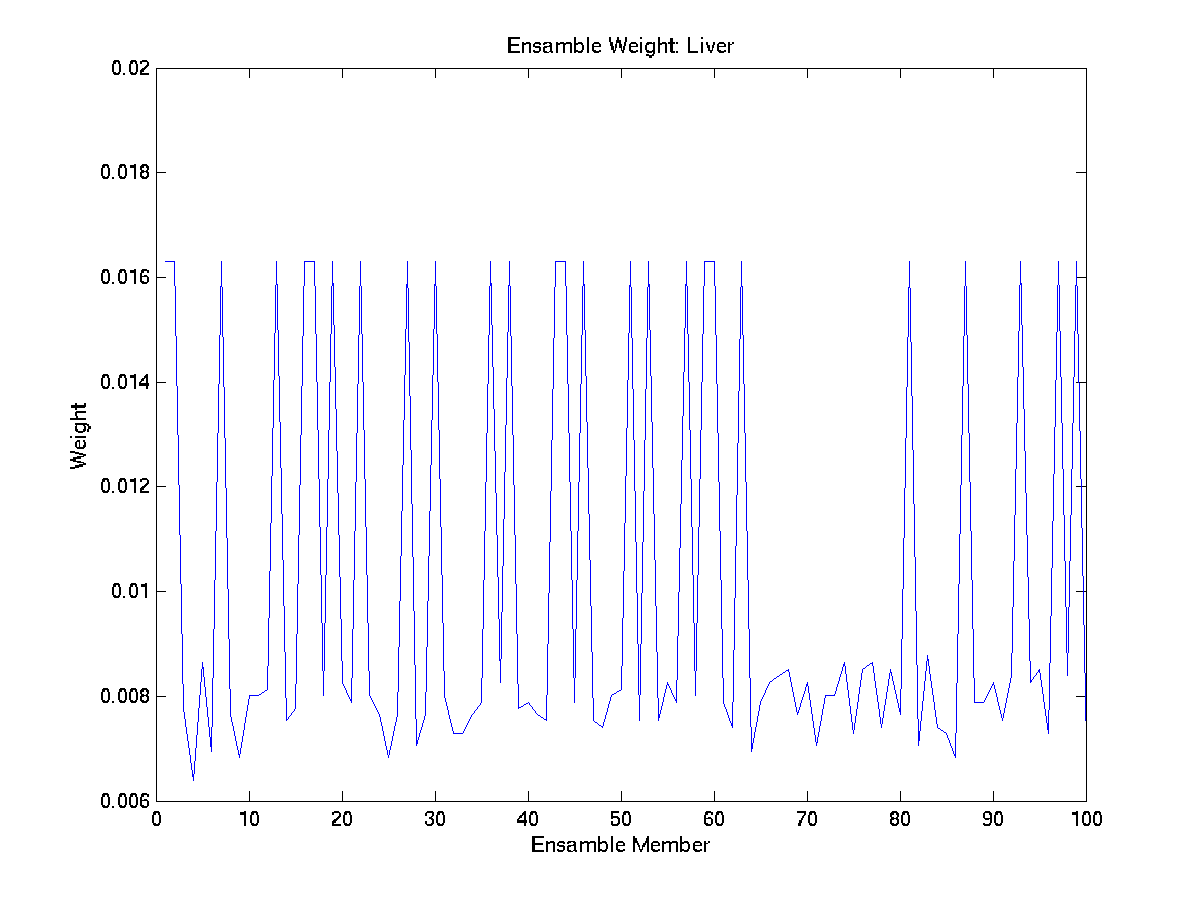
\includegraphics[width=\textwidth]{Liver_EnsambleWeight}
      \caption{Liver}
	\end{subfigure}%
	~
	\begin{subfigure}[b]{0.3\textwidth}
		\centering
		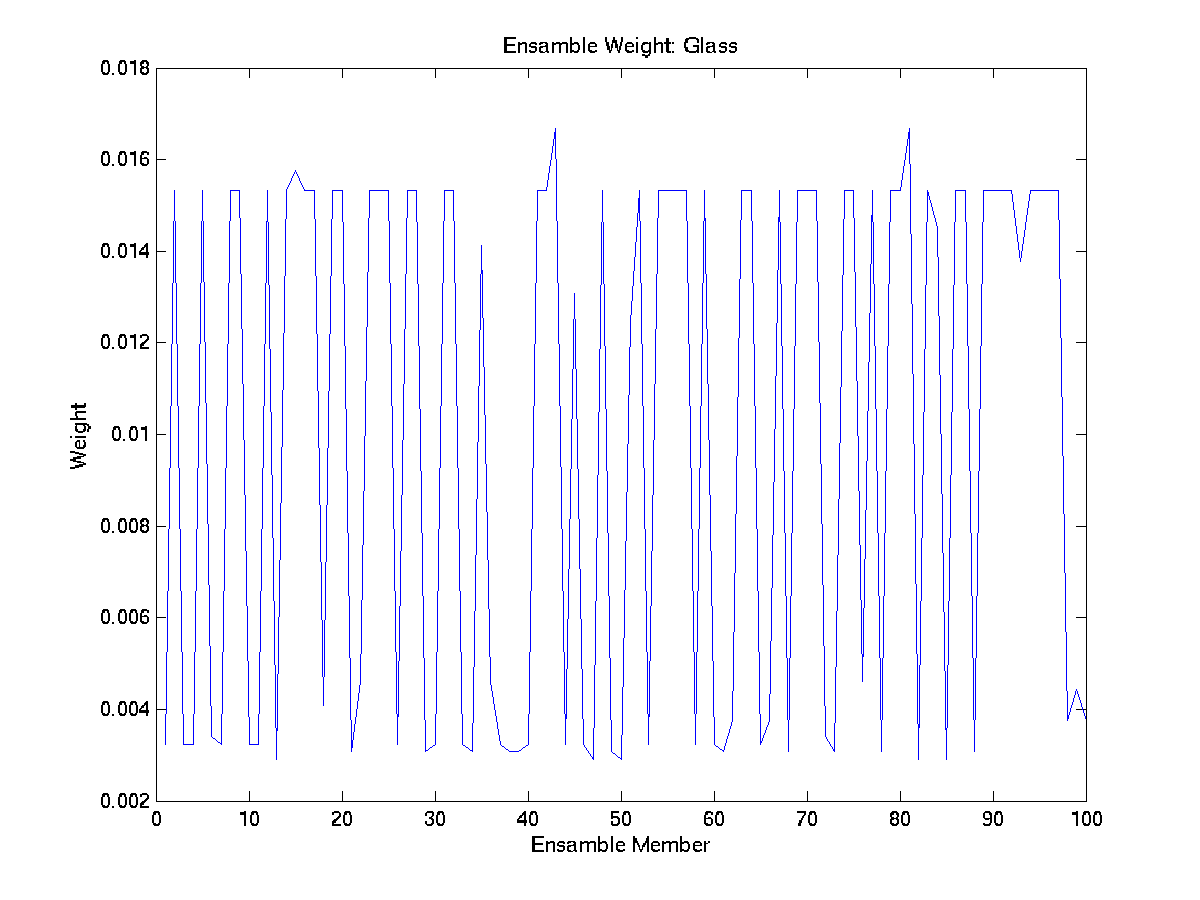
\includegraphics[width=\textwidth]{Glass_EnsambleWeight}
        \caption{Glass}
	\end{subfigure}	
    ~
	\begin{subfigure}[b]{0.3\textwidth}
		\centering
		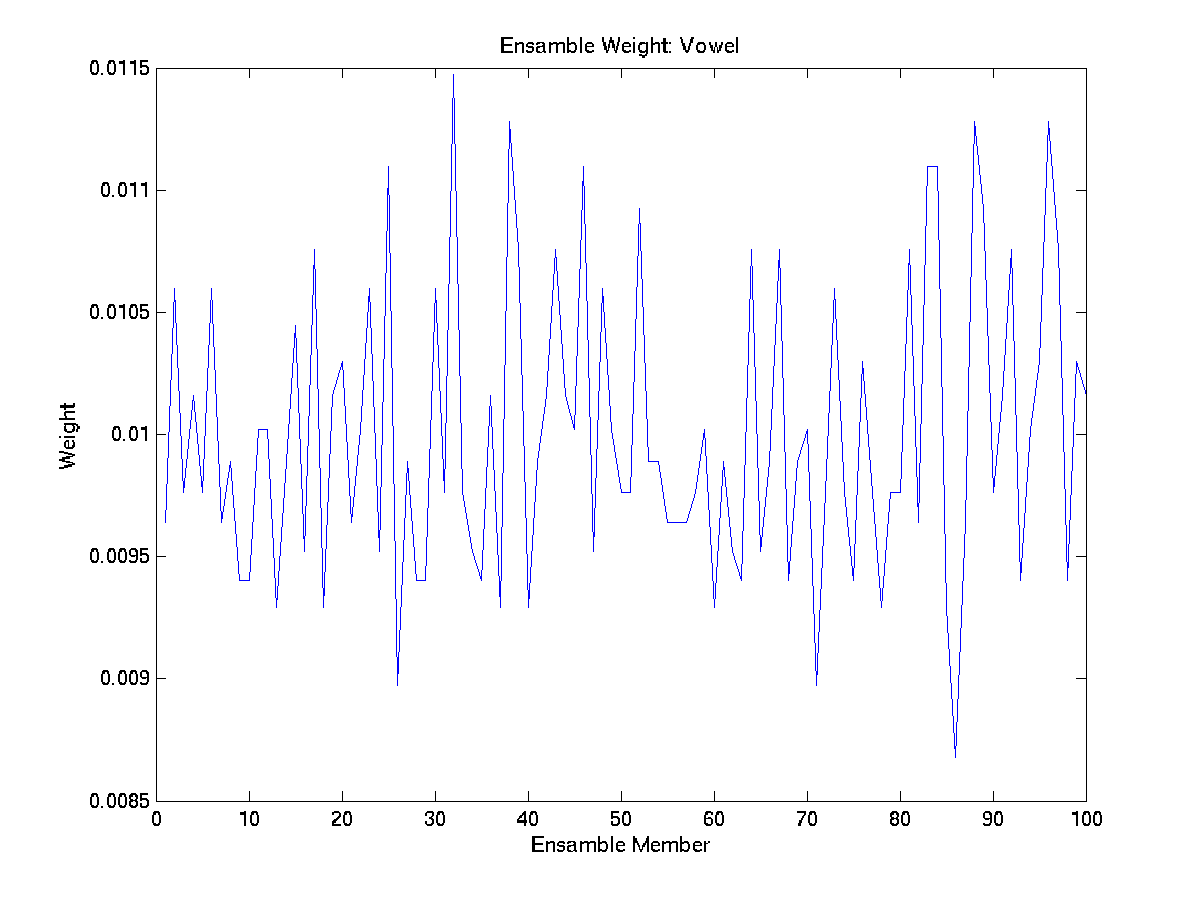
\includegraphics[width=\textwidth]{Vowel_EnsambleWeight}
        \caption{Vowel}
	\end{subfigure}%
	\caption{Distribution of Ensemble Weights}
	\label{fig:EnsambleWeights}
\end{figure*}
The confusion matrices of the AdaBoost ensemble classifiers are presented in Tables \ref{tab:AdaBoostConfusionLiver} - \ref{tab:AdaBoostConfusionVowel}.  
\begin{table}[h!]
\caption{Confusion Matrix for AdaBoost Ensemble (Liver)}
\label{tab:AdaBoostConfusionLiver}
\centering
\input{../Part2_Confusion_Liver.dat}
\end{table}
\begin{table}[h!]
\caption{Confusion Matrix for AdaBoost Ensemble (Glass)}
\label{tab:AdaBoostConfusionGlass}
\centering
\input{../Part2_Confusion_Glass.dat}
\end{table}
\begin{table}[h!]
\caption{Confusion Matrix for AdaBoost Ensemble (Vowel)}
\label{tab:AdaBoostConfusionVowel}
\centering
\input{../Part2_Confusion_Vowel.dat}
\end{table}
